\chapter{降低识别能耗的策略动态调整研究}
\par 在移动终端这个特殊的系统环境下,其中最大的限制就是能量有限。而在基于智能手机的行为识别整个过程中无论是内置传感器采集数据还是计算特征并对当前行为进行判决分类都会消耗较大的能量\cite{priyantha2010enabling}。因此我们有必要要研究在行为识别过程中降低手机能耗的方法,其最终目的就是通过权衡识别准确率和识别能耗,在保证一定准确率的前提下,尽可能降低在识别过程中智能手机的能耗。
\par 使用智能手机进行行为识别过程中,传感器采集运动数据,处理器计算特征向量以及运行分类算法对行为做判断识别都会消耗智能手机较多的能量。而在这一过程中,能耗的大小与传感器的采样率,采样时间,以及特征向量和分类算法的计算复杂度都有着直接的关系\cite{rachuri2011sociablesense}。另一方面,行为识别的识别准确率则取决于采集数据的充分性,特征集和分类算法的选择,所以准确率同样与采样率,采样时间,特征向量等的选择有直接关系\cite{ravi2005activity}。与此同时,对于不同的行为对数据量的要求,对特征集合的选择等都存在很大的不同\cite{raffa2010don},比如静止行为状态下,运动信息很少,对数据量的要求不高,而且也不存在频域特性,因此不需要在这段时间内以较高的采样率采集数据并计算频域等复杂特征,只需要运行较低的采样率监测过渡态行为是否发生即可。又比如在跑步状态下,其频域特征十分明显,且较容易识别,此时传感器只需要在窗口时间内的一部分时间采集数据就可以识别跑步状态,其他时间传感器进入休眠可以有效降低能耗。因此可以针对不同行为通过调节上述的一些变量,在较少影响准确率的情况下尽可能降低识别能耗。
\par 为研究降低识别能耗的策略调整方法,本章首先建立能耗和准确率的数学模型,研究二者与一些变量的函数关系,包括采样率,采样时间,特征集的选择等。与此同时,为了权衡识别准确率和识别能耗的关系,本文使用手机当前的能耗作为权衡系数,建立目标函数,为每一类行为求解最佳策略只需要求解相应目标函数的最优值即可,即转换为最优化问题。然后通过实验测量数据求解数学模型参数,进而求解每类行为的目标函数的最优解,从而获得每一种行为的最佳策略。最后提出一种结合行为识别结果和马尔科夫模型的行为转换矩阵的策略动态调整方法。

\section{数学模型}
\par 对于识别准确率和识别能耗的影响因素,本文考虑采样率,采样时间以及是否采用频域和自相关函数的特征作为变量研究准确率和能耗模型。本文中,采样率为传感器的数据采集速率,用$f$表示,采样时间使用窗口内的采样时间比例替代,如图\ref{window}所示,窗口时间长度为$T$,相邻窗口有50\%的重叠,其中有一定比例的窗口时间用于采集数据,比例用$\tau$表示。而是否使用频域和自相关函数的特征则可以使用0或1的离散变量表示,本文对其分为四种情况分别讨论。下面将讨论如何建立能耗与准确率模型,以及如何构建目标函数,进而为每类行为求解最佳策略。

\begin{figure}[ht]
\centering
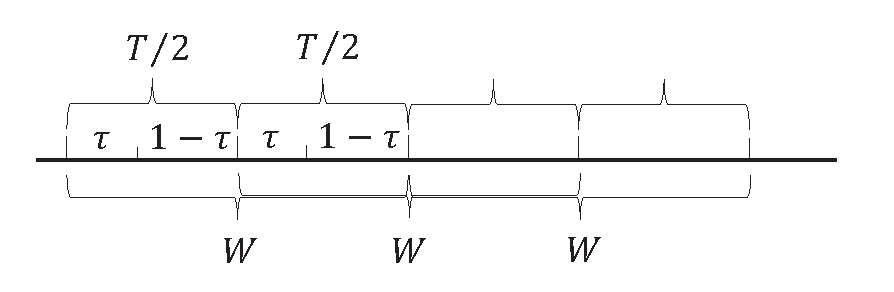
\includegraphics[width=8cm]{window.eps}
\caption{时间窗口示意图}\label{window}
\end{figure}

\subsection{能耗模型}
\par 使用智能手机执行行为识别过程中,能量损耗主要包括传感器的数据采集能耗和处理器的计算能耗两部分,因此能耗模型可以表示为:
\begin{equation}
	E(t) = E_S(t) + E_M(t)
\end{equation}
\par 首先是数据采集能耗,由于传感器是集成在智能手机内部,通常是由处理器负责充当传感器采集数据的ADC模块,传感器只负责运行采集模拟信号,处理器则根据指定的采样率采集离散信号,此外由处理器负责开启和关闭传感器。因此,数据采集能耗主要包括传感器运行能耗,处理器采集数据能耗以及传感器工作与休眠状态切换能耗。数据采集能耗的模型可以表示为:
\begin{equation}
	E_S(t) = (P_S\tau + P_A(f)\tau + P_{on-off}) \times t
\end{equation}
其中,$P_S$为传感器功率,$P_A$为处理器作为ADC模块采集数据时的功率,该功率与采样率有关,$P_{on-off}$为一定时间内处理器控制传感器切换工作和休眠状态时的等效平均功率,可以通过一段时间以确定频率周期性切换状态时能耗除以时间长度计算得到。
\par 其次是数据处理与计算能耗。行为识别过程中的数据处理和计算主要包括计算特征向量和运行分类算法。由于本文中,特征集包括时域、频域和自相关函数特征三个方面,而时域特征可以通过时域信号直接计算,计算量较小,能耗较低,因此本文方案总是使用时域特征,不再将其作为一个变量。与此同时,频域和自相关函数的特征需要对信号做快速傅里叶变换和求解自相关函数,计算量较大,因此本文将是否使用这两个类型的特征作为两个离散变量考虑进能耗模型中,而根据频域信号和自相关函数计算相应特征则过程十分简单,能耗相对较小,本文中将其忽略。因此数据处理能耗可以表示为:
\begin{equation}
	E_M(t) = (\mu E_{FFT} + \lambda E_{ACF} + E_C) \times \theta \times t
\end{equation}
其中,$E_{FFT}$和$E_{ACF}$分别表示计算单次FFT和ACF所消耗的能量,$\mu$,$\lambda$取值为0或1,表示不使用或使用频域或自相关函数的特征,$E_C$表示运行分类算法对行为实例分类时的能耗。$\theta$表示单位时间内执行识别分类的次数,因为在一个时间窗口内执行一次识别,需要计算一次FFT和ACF,用于提取频域和自相关函数的特征,因此数据处理的等效平均功率即可以表示单次执行分类的所有能耗乘以单位时间内执行分类的次数。

\subsection{准确率模型}
\par 行为识别的准确率同样也是主要受到来自本文所提到的四个变量的影响,即采样率,采样时间比例,是否采用频域和自相关函数的特征。对于采样率和采样时间比例,二者均为连续变量,本文重点研究准确率与二者的函数关系,而对于是否使用频域和自相关函数的特征则是两个离散值,因此在本文中分成四种不同情况讨论准确率模型。下面以使用全部特征,即包含频域和自相关函数特征为例说明准确率模型,其他三种情况与之类似。
\par 首先识别准确率是受到采样率和采样时间的影响,但是它与二者没有确定的显式函数关系,其次不同行为的识别准确率对采样率和采样时间的敏感程度也会有所不同\cite{wang2009framework},比如对于静止状态的行为,由于其运动传感器的数据在一定时间内变化不大,采样率的大小对其影响较小,而对于快速运动状态,其识别准确率则很大程度地依赖采样率的大小。所以本文首先建立识别准确率与采样率和采样时间比例的数学模型,然后针对每一类行为通过实验训练集数据的识别结果拟合数学模型参数,从而获得最适合该行为的函数关系模型。

\begin{figure}[!htb]
    \centering
    \subfloat[行走状态下的识别准确率]{
    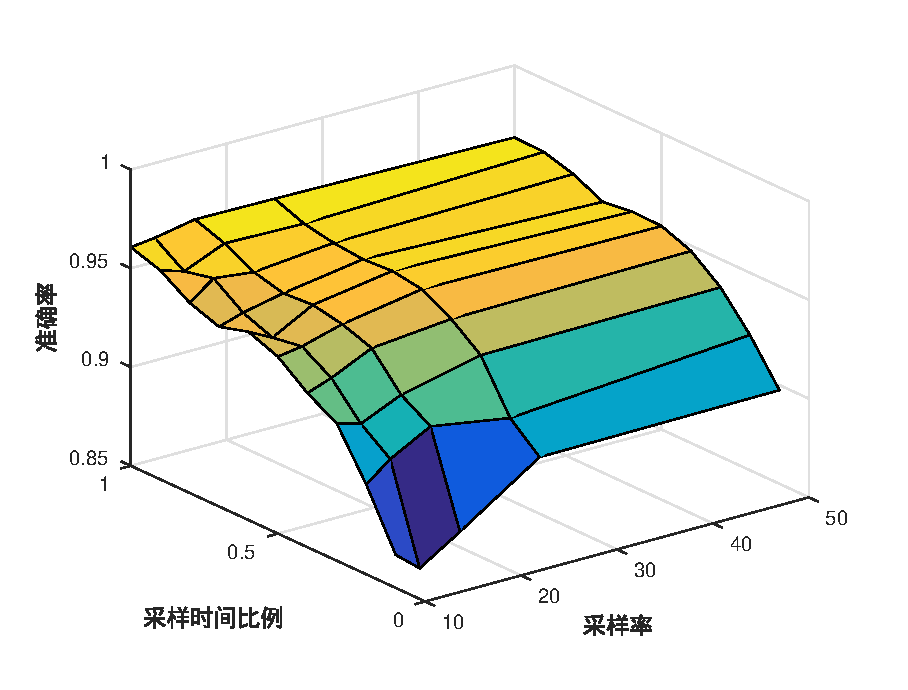
\includegraphics[width=0.45\textwidth]{walk_precision.eps}}
    \subfloat[跑步状态下的识别准确率]{
    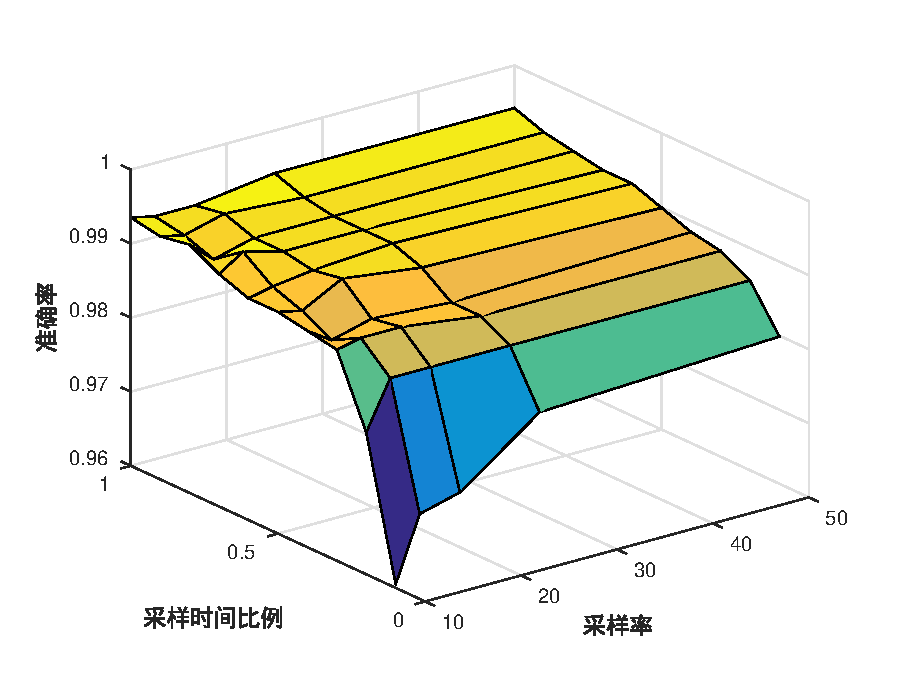
\includegraphics[width=0.45\textwidth]{run_precision.eps}}
    \caption{识别准确率与采样率和采样时间比例的关系}\label{precision}
\end{figure}

\par 图\ref{precision}(a)和\ref{precision}(b)分别表示行走状态和跑步状态下,实验训练集数据识别准确率与采样率和采样时间比例的关系。从图中我们可以看出准确率与两个变量之间基本都是成负指数函数关系。因此本文考虑为识别准确率建立以下数学模型:
\begin{equation}
	Precision(i) = exp(-\frac{\alpha_i}{f} - \frac{\beta_i}{\tau})
\end{equation}
其中,$\alpha_i$,$\beta_i$为待拟合参数,$f$表示采样率,$\tau$表示采样时间比例,$i$表示某一类行为$i$。
\par 在建立识别准确率的数学模型以后,根据不同采样率和采样时间比例的训练集数据即可拟合该数学模型,从而获得相应的模型参数。
\subsection{目标函数}
\par 本部分研究的根本目标是为行为识别选择一种策略,使得在保证一定准确率的前提下,尽可能降低在识别过程中的各部分能量损耗。但是识别准确率和能耗存在明显的矛盾关系,因此选择最佳策略需要在能耗与准确率之间寻找一个最佳的权衡。为了更好地考虑和权衡二者的关系,本文通过建立目标函数将准确率和能耗统一在一个函数中。
\par 建立目标函数首先需要考虑的是权衡系数问题,即二者不同的重要程度。本文考虑将智能手机的电量离散化为若干等级,并使用当前电量所处的等级所谓权衡系数,当电量充足时提升准确率在目标函数的重要程度,电量较少时则提升能耗在目标函数中的重要程度。其次是准确率和能耗的数值归一化问题。准确率是一个比例,其数值大部分分布在0.8到1.0之间,而能耗的数值则是一个实数,代表时间的耗电量,为了更好权衡二者关系需要将其数值做归一化处理。本文考虑为准确率设定可接受的准确率最低阈值$Precision_{low}$,并将准确率从$Precision_{low}$到1.0的数值映射到0到1.0之间,对于准确率低于阈值的情况则变换为负无穷,即不可接受的准确率。对于能耗的归一化,本文考虑通过将能耗数值除以“最强策略”的能耗值做归一化。所谓“最强策略”即使用可设定的最高采样率,100\%的采样时间比例以及使用频域和自相关函数的特征情况。最后是离散变量问题,即是否使用频域和自相函数特征是两个独立且离散的变量,直接将其放入目标函数会对求解最优化问题造成困难,因此在构建目标函数时,本文同之前的考虑相同,将其作为四种情况分类讨论,在求解最优化问题时,从四个求解得到的最优目标函数值中再择最优即可。
\par 确定目标函数以后,为每类行为选择最佳策略就可以转换为求解目标函数最优值的最优化问题,而优化变量即为待求解的最佳策略。其中最优化问题可以表示为:
\begin{equation}
  \begin{array}{ll}
    min  & z=\{(1-\varphi (battery)) \frac{E_T}{E_{max}} - \varphi (battery) \frac{Precision(i) - Precision_{low}}{1 - Precision_{low}}\} \\
    \\
    s.t. & \begin{array}[t]{rll}
             \mu 			 &  =    & 0|1 \\
             \lambda         &  =    & 0|1  \\
             Precision(i)    & \geq  & Precision_{low}
           \end{array}
  \end{array}
\end{equation}

其中,$E_{max}$表示“最强策略”下的能耗,$Precision_{low}$表示准确率的最低阈值,也是可以接受的最低识别准确率。$\mu, \lambda$表示是否使用频域和自相关函数特征,此最优化问题根据$\mu, \lambda = 0|1$分为四类情况分别求解,然后在其中取最优值。该最优化问题的解即为对应行为的最佳识别策略。


\section{模型求解}
\par 通过上一小节建立的数学模型以及目标函数,本文是通过求解一个关于目标函数的最优化问题为每类行为计算其对应的最佳识别策略。本小节将详细介绍上述各数学模型参数的具体求解过程。首先是对于能耗模型,本文通过开发手机应用,在一系列的固定时间段内采用设定的采样率采集数据,以及一系列固定次数的特征计算,然后通过线性拟合的方式求解能耗模型的各个参数。其次对于准确率模型,本文将之前采集的数据做下采样或截断处理,使其满足一系列指定采样率和采样时间比例,然后通过对其分类求取的准确率对建立的准确率数学模型做曲面拟合,求取模型中的参数值。最后在获得具体模型以后,即可以通过求解目标函数最优值为每一类行为获取最佳策略。

\subsection{能耗模型求解}
\par 能耗模型的求解需要实际测量智能手机在采集数据和计算特征等时所消耗的能量。为此,本文以Android操作系统为例,编写手机应用,执行数据采集或者数据处理等逻辑,进而测量该过程中的能量损耗。在手机应用中数据采集或数据处理能耗主要以耗电量的形式表示,而为了更为精确地测量应用的耗电量,Android系统提供了dumpsys工具可以用于查看系统服务信息和状态,通过该工具的battery命令即可以查看应用一段时间内的耗电量。battery命令可以给出手机上每个进程的各个硬件的详细耗电量,包括处理器,WiFi和传感器等,因此本文使用它可以很精确测量数据采集和数据处理的各部分能耗。
\par 首先需要明确能耗测量实验设定,本文使用Google的Nexus5智能手机运行能耗测量应用,该应用可设定数据采样率,采样时间比例以及计算快速傅里叶变换或自相关函数的次数,并测量相应的手机耗电量,单位是mAh。首先是在数据采集部分,本文设定采样率为15Hz, 25Hz, 40Hz, 50Hz, 100Hz;采样时间比例设定为100\%,50\%,0\%。由于传感器运行能耗可以单独测量,但是处理器能耗则包括数据采集,控制传感器工作状态切换以及其他控制逻辑的多方面的能耗,无法单独测量,因此本文中首先设定100\%的采样时间比例可以使得在没有处理器控制传感器切换传感器工作状态时干扰的情况下研究不同采样率的数据采样能耗与采样率的关系,然后设置50\%的采样时间比例所测得结果,通过减去对应一半时间用于数据采样的能耗就可以得到处理器控制传感器切换工作状态的能耗,最后设置0\%的采样时间比例是为了测量其他控制逻辑的能耗,使得在计算各部分能耗时减去该部分能耗。测量实验在不同的采样率和采样时间比例的情况下,设定测量时间为1到5分钟,五个时间段,分别统计应用中传感器和处理器的能耗,每一组实验设定情况下重复测量5次,求取平均值作为该实验设定实验参数下的能耗结果,最后通过拟合能耗与时间的关系计算各部分的耗能功率。

	(1) 传感器功率
\par 传感器作为智能手机内置硬件,其能耗可以单独测量,因此计算较为简单。表格\ref{100_energy}和\ref{50_energy}为实验测量得到的传感器能耗。

\begin{table}[htb]
    \centering
    \caption{100\%采样时间情况下传感器能耗(单位:毫安时$(mAh)$)}\label{100_energy}
    \begin{tabular}{cccccc}
    \toprule
     $T(min)$ & 1 & 2 & 3 & 4 & 5 \\
    \midrule
    15Hz & 0.00321 & 0.00655 & 0.0099 & 0.0132 & 0.0166 \\
    25Hz & 0.00319 & 0.00655 & 0.00988 & 0.0132 & 0.0166 \\
    40Hz & 0.00321 & 0.00651 & 0.0197 & 0.0132 & 0.0166 \\
    50Hz & 0.00325 & 0.00654 & 0.0197 & 0.0132 & 0.0166 \\
    100Hz & 0.0032 & 0.00659 & 0.0099 & 0.0132 & 0.0164 \\
    \bottomrule
    \end{tabular}
 \end{table}

 \begin{table}[htb]
    \centering
    \caption{50\%采样时间情况下传感器能耗(单位:毫安时$(mAh)$)}\label{50_energy}
    \begin{tabular}{cccccc}
    \toprule
     $T(min)$ & 1 & 2 & 3 & 4 & 5 \\
    \midrule
    15Hz & 0.00159 & 0.00324 & 0.00491 & 0.00641 & 0.0081 \\
    25Hz & 0.00159 & 0.00327 & 0.00485 & 0.0067 & 0.00823 \\
    40Hz & 0.00158 & 0.00318 & 0.00483 & 0.00644 & 0.00815 \\
    50Hz & 0.0016 & 0.00322 & 0.0049 & 0.00641 & 0.00815 \\
    100Hz & 0.00159 & 0.00325 & 0.00482 & 0.00656 & 0.008 \\
    \bottomrule
    \end{tabular}
 \end{table}


\par 从数据中可以明显看出传感器的能耗与采样率无关,与时间成正比。因为与采样率无关,这里以50Hz采样率情况下的数据为例,进行线性拟合后如图\ref{sensor_energy}所示,可以发现明显的正比关系。通过线性拟合求取斜率可以计算出传感器的功率为$P_S = 3.4 \times 10^{-3} (mAh/min)$。

\begin{figure}[htb]
\centering
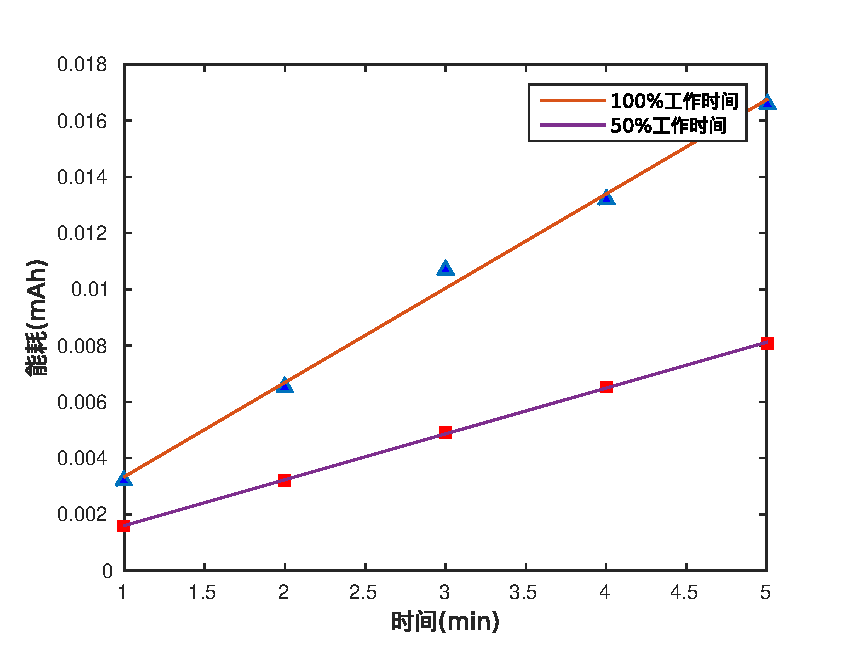
\includegraphics[width=0.5\textwidth]{sensor_energy.eps}
\caption{50Hz的采样率情况下传感器能耗与时间的关系}\label{sensor_energy}
\end{figure}

\begin{figure}[!htb]
    \centering
    \subfloat[15Hz采样率情况下的能耗]{
    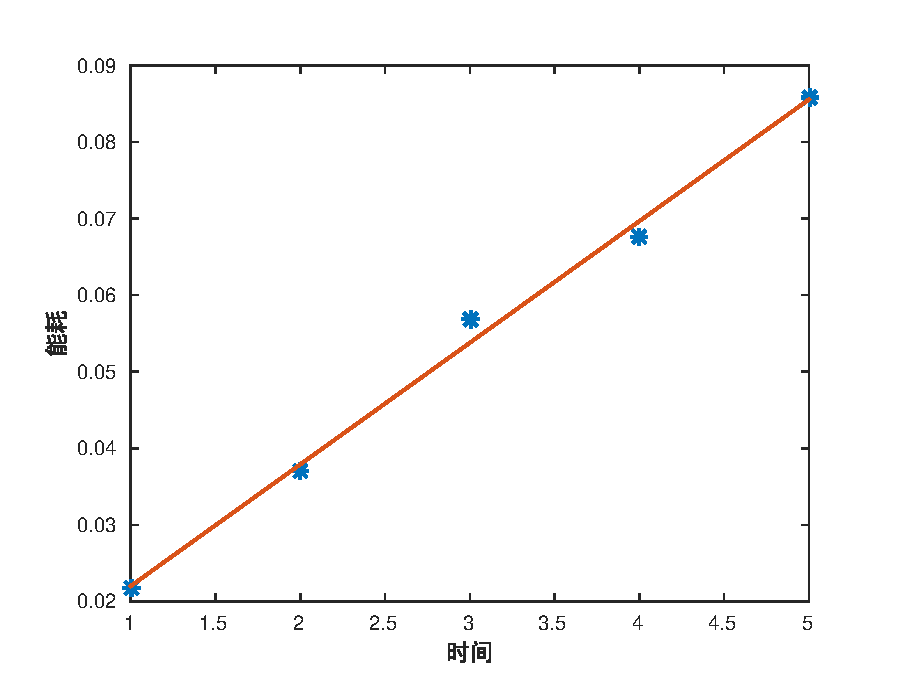
\includegraphics[width=0.3\textwidth]{100_sample_15Hz.eps}}
    \subfloat[25Hz采样率情况下的能耗]{
    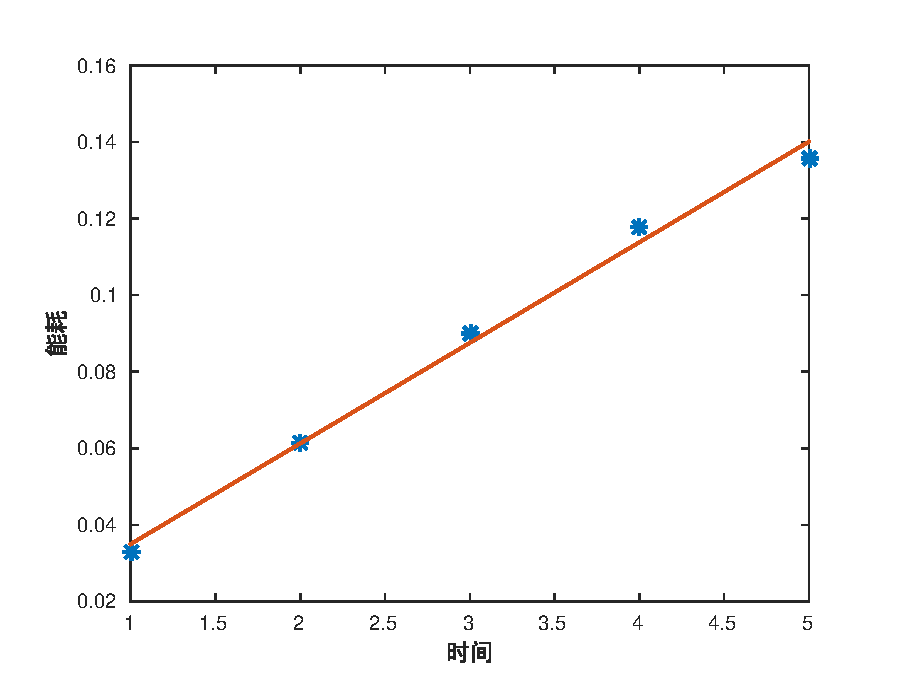
\includegraphics[width=0.3\textwidth]{100_sample_25Hz.eps}}
    \subfloat[40Hz采样率情况下的能耗]{
    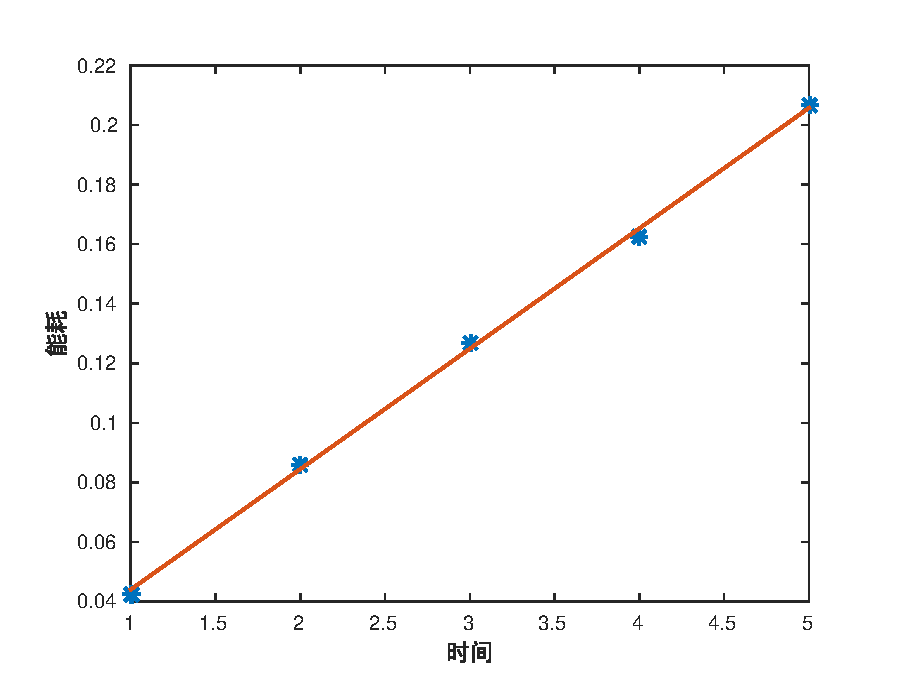
\includegraphics[width=0.3\textwidth]{100_sample_40Hz.eps}}
    \subfloat[50Hz采样率情况下的能耗]{
    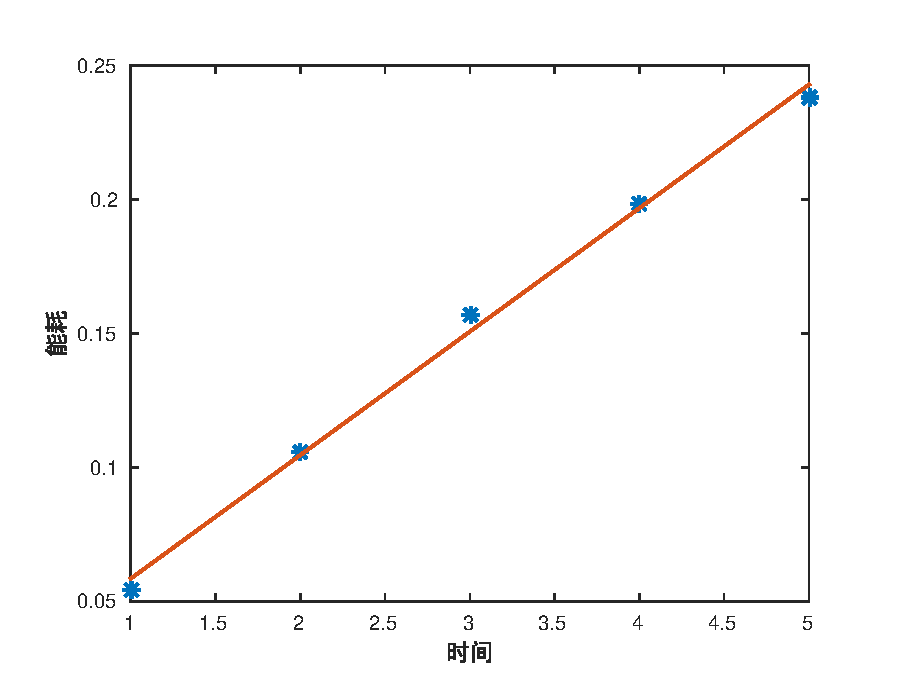
\includegraphics[width=0.3\textwidth]{100_sample_50Hz.eps}}
    \subfloat[100Hz采样率情况下的能耗]{
    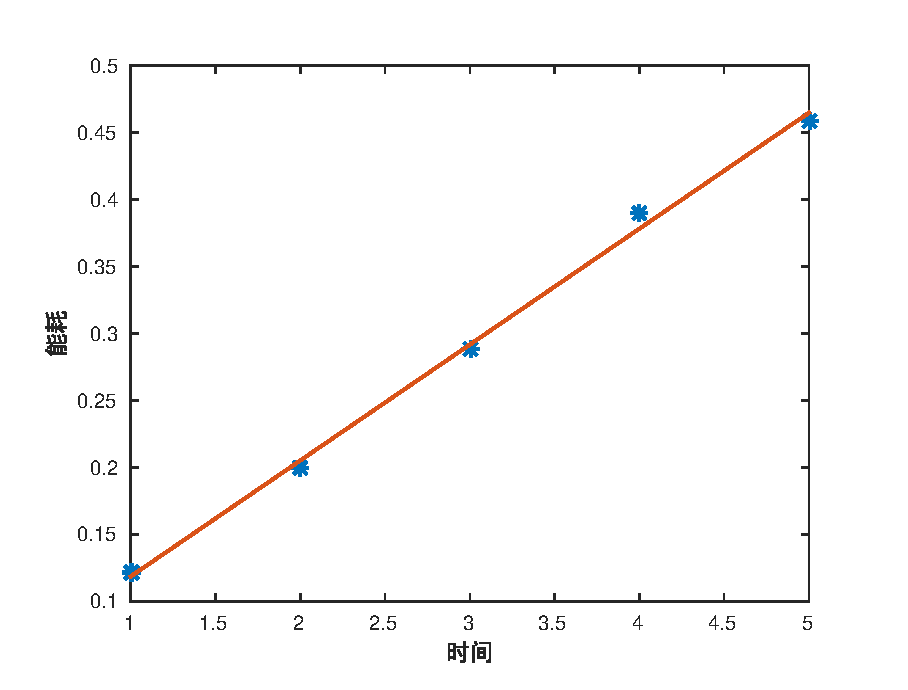
\includegraphics[width=0.3\textwidth]{100_sample_100Hz.eps}}
    \caption{100\%采样时间以及各采样率情况下处理器的数据采集能耗与时间的关系}\label{sample}
\end{figure}


	(2) 处理器的数据采集功率

\par 在智能手机内部由处理器充当传感器ADC模块的角色,负责数据采集。本文首先设定100\%的数据采样时间比例,即持续采集数据,避免了处理器在控制传感器切换状态时带来的能耗方面的干扰。然后在5个采样率的实验设定情况下,测量5种时间段内处理器的数据采集能耗,多次测量结果的平均能耗最为该实验设定的结果,研究与时间的关系如图\ref{sample}(a)-(e)所示。


\par 从图\ref{sample}(a)-(e)中可以看出,在每个采样率的情况下平均能耗都与时间成正比,即数据采集功率是保持恒定的。因此本文通过线性拟合可以计算得到每个采样率情况下的数据采集功率,而数据采集功率与采样率的关系如图\ref{p_sample_rate}所示。从图可以看出,数据采集功率同样与采样率也是成正比,经过线性拟合,可以计算得到功率与采样率的关系,其正比系数为$\alpha = 8.3962 \times 10^{-4} \quad mAh/min*Hz$。

\begin{figure}[!htb]
\centering
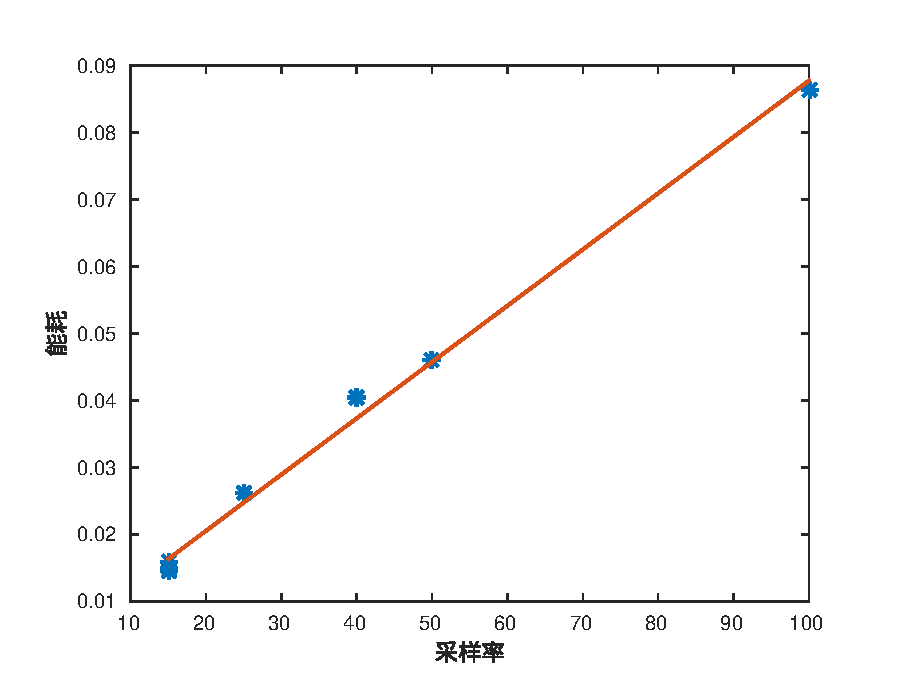
\includegraphics[width=0.5\textwidth]{p_sample_rate.eps}
\caption{处理器数据采集功率与采样率的关系}\label{p_sample_rate}
\end{figure}



	(3) 处理器的控制状态切换等效平均功率


\begin{figure}[!htb]
    \centering
    \subfloat[50\%的时间比例情况下采集数据时处理器的能耗]{
    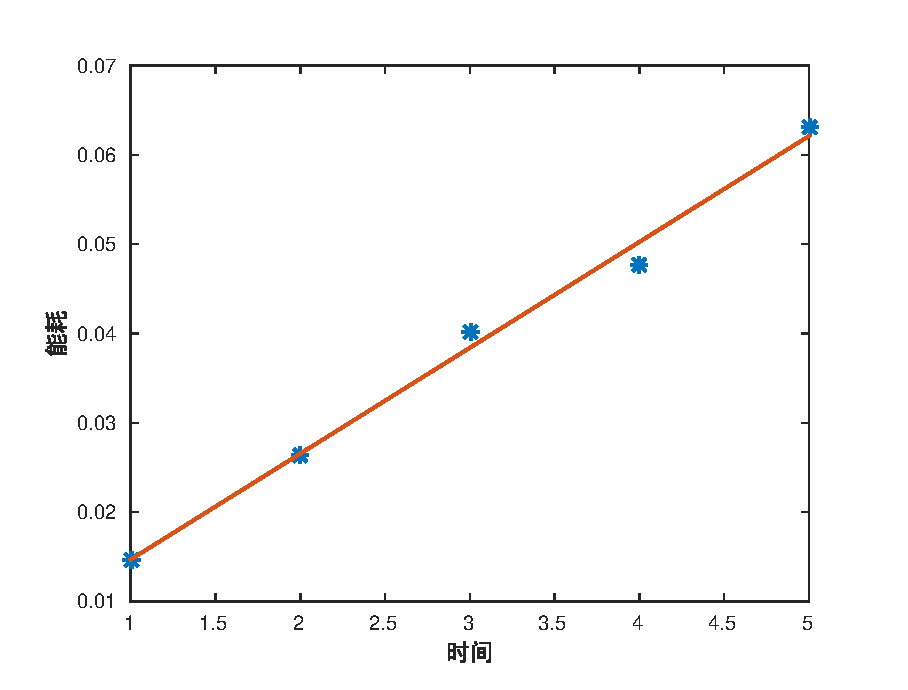
\includegraphics[width=0.45\textwidth]{50_sample_15Hz.eps}}
    \subfloat[处理器控制传感器状态切换时的能耗]{
    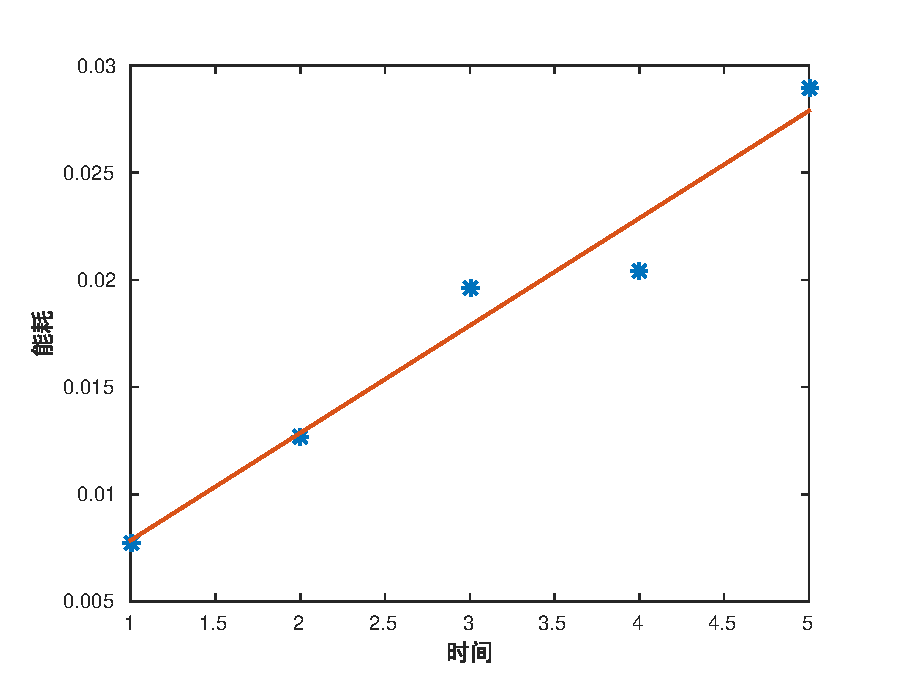
\includegraphics[width=0.45\textwidth]{on-off_p.eps}}
    \caption{处理器能耗与时间的关系}\label{on-off}
\end{figure}

\par 由于处理器的多任务性,无法单独测量控制状态切换功率,因此本文设定50\%的采样时间比例以及15Hz测量处理器能耗,并且设定没2.5s传感器状态切换一次,即一个开关的周期,该时间与行为识别中执行一次识别判定的时间相同。如图\ref{on-off}(a)所示为50\%的时间比例情况下采集数据时处理器的能耗与时间的关系。通过从中减去50\%的时间内数据采集的能耗(该能耗可以通过数据采集功率乘以数据采集时间计算得到)即可以获得控制传感器工作状态切换能耗。在15Hz的采样率下,控制状态切换的能耗与时间的关系如图\ref{on-off}(b)所示。此外,在其他采样率下可以通过相同方法计算处理器控制传感器状态切换能耗,其结果在误差范围以内与之相同。从\ref{on-off}(b)图中可以看出,该能耗与时间正比,虽然在每次发生状态切换时才会有能耗,但是通过线性拟合可以计算其等效平均功率,这也有助于能耗模型的计算。最后控制状态切换等效平均功率为:$P_{on-off} = 3.6 \times 10^{-3} (mAh/min)$。在当前实验设定情况下,每分钟传感器的状态切换24次,因此每次切换的能耗为$E_{on-off} = 1.5 \times 10^{-3}(mAh)$

	(4) 处理器的数据处理等效平均功率

\par 由于本文只考虑是否使用频域或自相关函数特征作为调节变量,因此只测量处理器在计算快速傅里变换(FFT)和自相关函数(ACF)的能耗,而特征计算与之相比数值较小,可以忽略不计。本实验通过设定一系列的执行次数测量处理器能耗,其结果如表格\ref{compute_energy}所示。图\ref{fft_acf}表示处理器计算FFT和ACF的能耗与执行次数的关系,从中也可以看出明显正比关系。

\begin{table}[htb]
    \centering
    \caption{处理器计算FFT和ACF的能耗(单位:毫安时$(mAh)$)}\label{compute_energy}
    \begin{tabular}{ccccccccccc}
    \toprule
    执行次数 & 1000 & 2000 & 3000 & 4000 & 5000 & 6000 & 7000 & 8000 & 9000 & 10000 \\
    \midrule
    FFT & 0.111 & 0.335 & 0.640 & 0.743 & 1.043 & 1.42 & 1.56 & 1.72 & 1.97 & 2.715 \\
    ACF & 0.084 & 0.152 & 0.226 & 0.299 & 0.362 & 0.408 & 0.569 & 0.596 & 0.809 & 0.883 \\
    \bottomrule
    \end{tabular}
 \end{table}

\begin{figure}[htb]
\centering
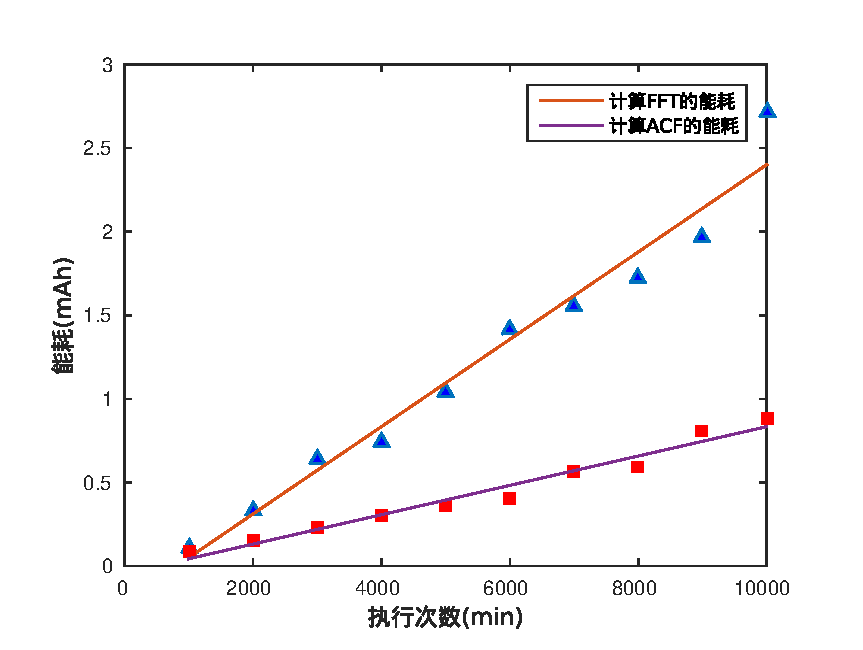
\includegraphics[width=0.5\textwidth]{fft_acf.eps}
\caption{处理器计算FFT和ACF的能耗与执行次数的关系}\label{fft_acf}
\end{figure}

通过线性拟合,可以得到单次计算傅里叶变换和自相关函数的能耗分别为$E_{FFT} = 0.30 \times 10^{-3} mAh, E_{FFT} = 0.10 \times 10^{-3} mAh$。为了便于计算,本文使用同一计量单位,为此分别计算其等效平均功率,即乘以单位时间内执行计算次数 $\theta = 24$, 即2.5s执行一次计算,与之前的进行一次识别判定相同, 其等效平均功率为:$P_{FFT} = 7.20 \times 10^{-3} mAh/min, E_{FFT} = 2.40 \times 10^{-3} mAh/min$。

\subsection{准确率模型求解}
\par 首先是实验设定,本文使用之前采集的50Hz采样率,100\%时间采样的情况下所获取的训练数据集。实验设定5Hz, 10Hz, 16.7Hz, 25Hz, 50Hz五个采样率,10\%到100\%十个采样时间比例。然后对原始训练数据集进行下采样和数据窗口内截断等方法获取实验设定中采样率和采样时间各个组合设定条件下的数据集。最后针对每个数据集,根据是否使用频域和自相关函数特征分为四组,分别提取规定特征并进行分类实验,最终获取分类的准确率结果。

\begin{figure}[!htb]
    \centering
    \subfloat[实际的行走识别准确率]{
    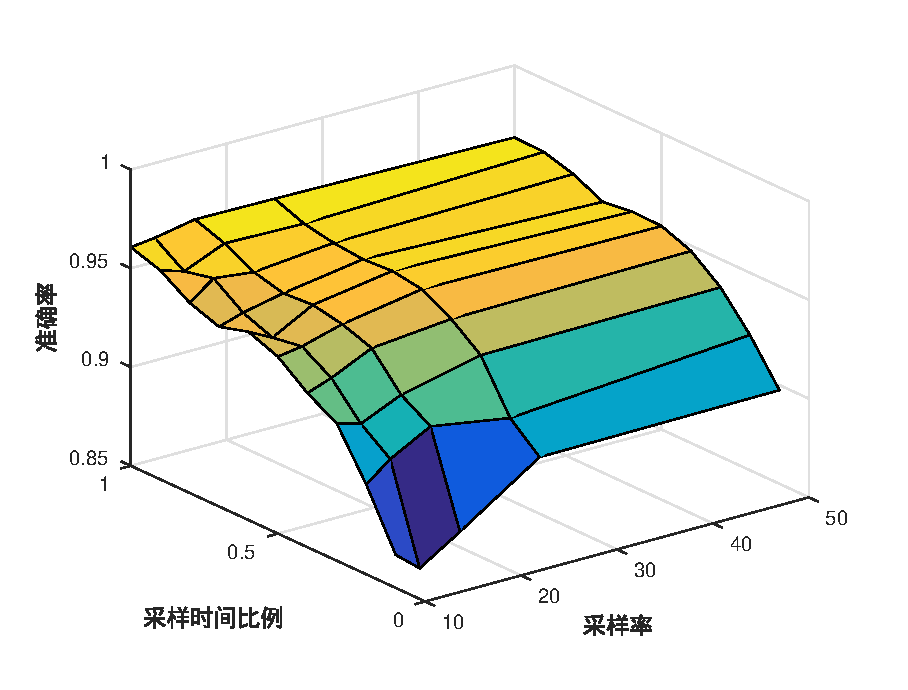
\includegraphics[width=0.45\textwidth]{walk_precision.eps}}
    \subfloat[拟合的行走识别准确率]{
    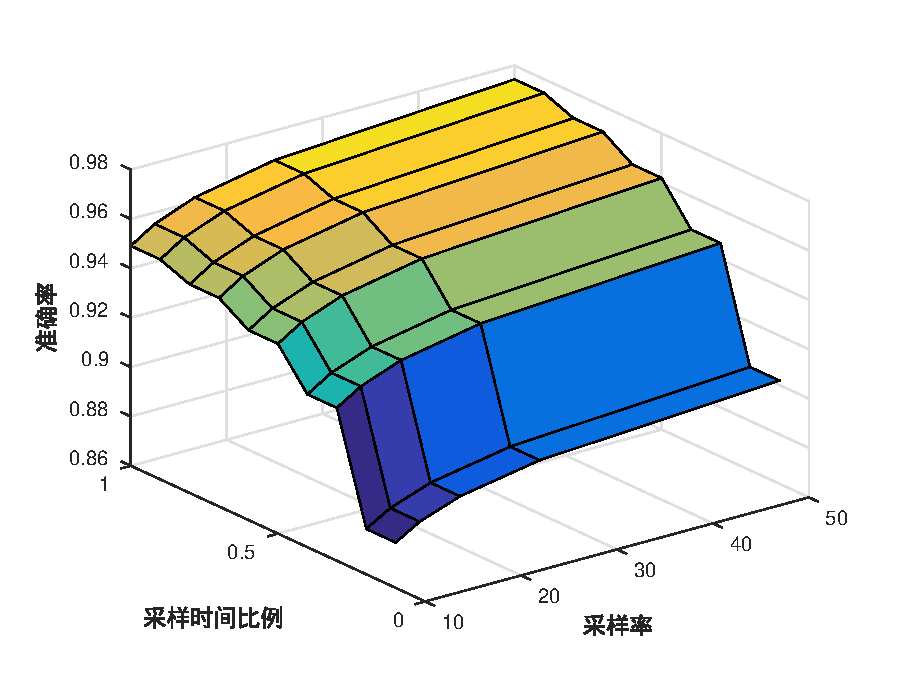
\includegraphics[width=0.45\textwidth]{walk_precision_fit.eps}}
    \caption{行走状态下的识别准确率与采样率以及采样时间比例之间的关系}\label{fit_precision}
\end{figure}

\par 图\ref{fit_precision}(a)为在使用频域和自相关函数特征的情况下,行走准确率与采样率和采样时间比例的关系,本文考虑使用曲面拟合的方法求解准确率模型中的参数。拟合后的效果如图\ref{fit_precision}(b)所示,从图中可以看出拟合后的曲面可以较好地反映出准确率与两个变量的函数关系。同样地,对于其他行为在不同的特征选择范围情况下也可以通过曲面拟合并求解参数,最后求解的参数和拟合残差结果如表格\ref{fit_result}所示。

\begin{table}[htb]
    \centering
    \caption{处理器计算FFT和ACF的能耗(单位:毫安时$(mAh)$)}\label{fit_result}
    \begin{tabular}{ccccccc}
    \toprule
    特征选择范围 &  参数 & 静止 & 行走 & 跑步 & 上楼 & 下楼\\
    \midrule
    \multirow{3}{2cm}{使用全部特征} & $\alpha$ & 0.112725 & 0.328838 & 0.041147 & 0.142354 & 0.10464 \\
    & $\beta$ & 0.001404 & 0.009677 & 0.001975 & 0.022183 & 0.029299 \\
    & 残差 & 0.000536 & 0.005263 & 0.000677 & 0.031337 & 0.078689 \\
    \midrule
    \multirow{3}{2cm}{使用时域和频域特征} & $\alpha$ & 0.125692 & 0.344354 & 0.041036 & 0.185501 & 0.04843 \\
    & $\beta$ & 0.001725 & 0.009621 & 0.002006 & 0.021795 & 0.029252 \\
    & 残差 & 0.000667 & 0.004364 & 0.000897 & 0.032815 & 0.06864 \\
    \midrule
    \multirow{3}{2cm}{使用时域和频域特征} & $\alpha$ & 0.099123 & 0.376837 & 0.056402 & 0.369427 & 0.128952 \\
    & $\beta$ & 0.001372 & 0.010081 & 0.001988 & 0.022509 & 0.029771 \\
    & 残差 & 0.000405 & 0.006223 & 0.000679 & 0.02864 & 0.057017 \\
    \midrule
    \multirow{3}{2cm}{仅使用时域特征}  & $\alpha$ & 0.116857 & 0.520193 & 0.067148 & 0.593838 & 0.616581 \\
    & $\beta$ & 0.001653 & 0.010415 & 0.c001989 & 0.021963 & 0.029101 \\
    & 残差 & 0.000669 & 0.009035 & 0.000756 & 0.029607 & 0.041895 \\
    \bottomrule
    \end{tabular}
\end{table}
\par 从表格\ref{fit_result}中可以看出拟合残差都较小,基本上都在5\%以内,这说明本文的准确率数学模型可以很好地刻画准确率与采样率和采样时间比例之间的关系。

\begin{figure}[!htb]
    \centering
    \subfloat[静止状态的目标函数]{
    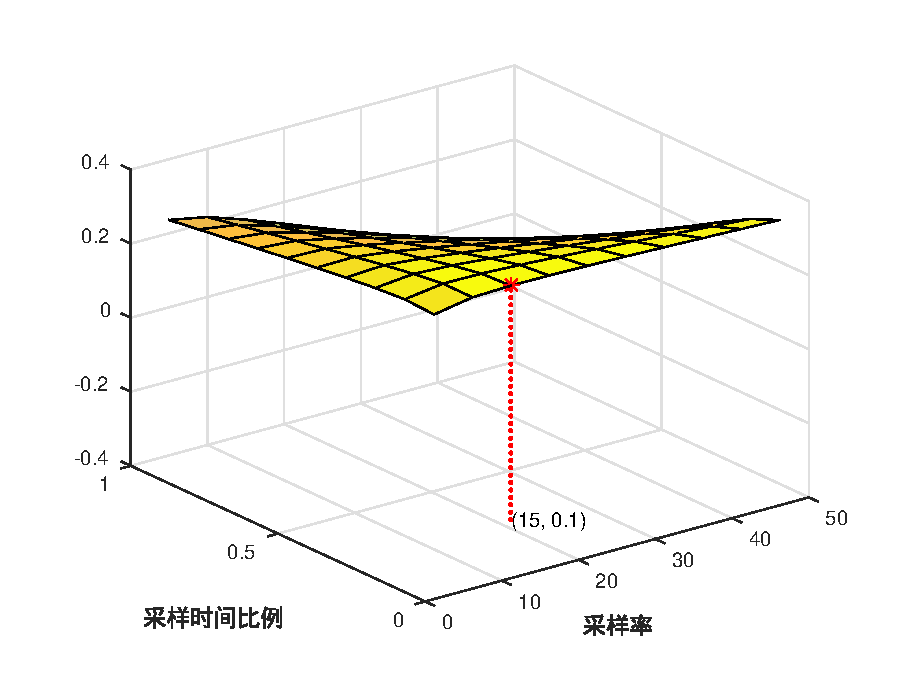
\includegraphics[width=0.3\textwidth]{object_static.eps}}
    \subfloat[行走状态的目标函数]{
    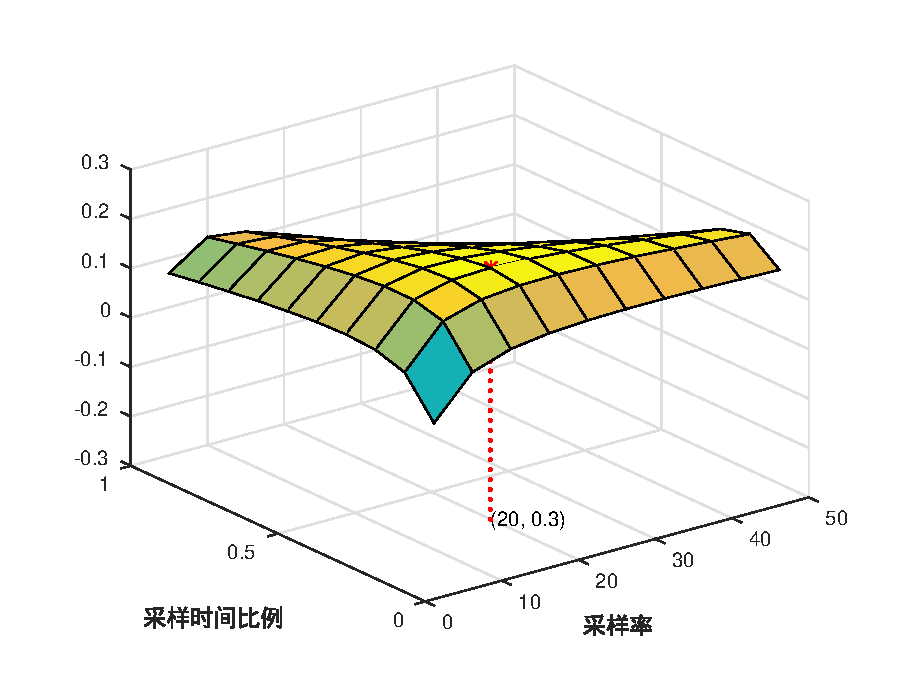
\includegraphics[width=0.3\textwidth]{object_walk.eps}}
    \subfloat[跑步状态的目标函数]{
    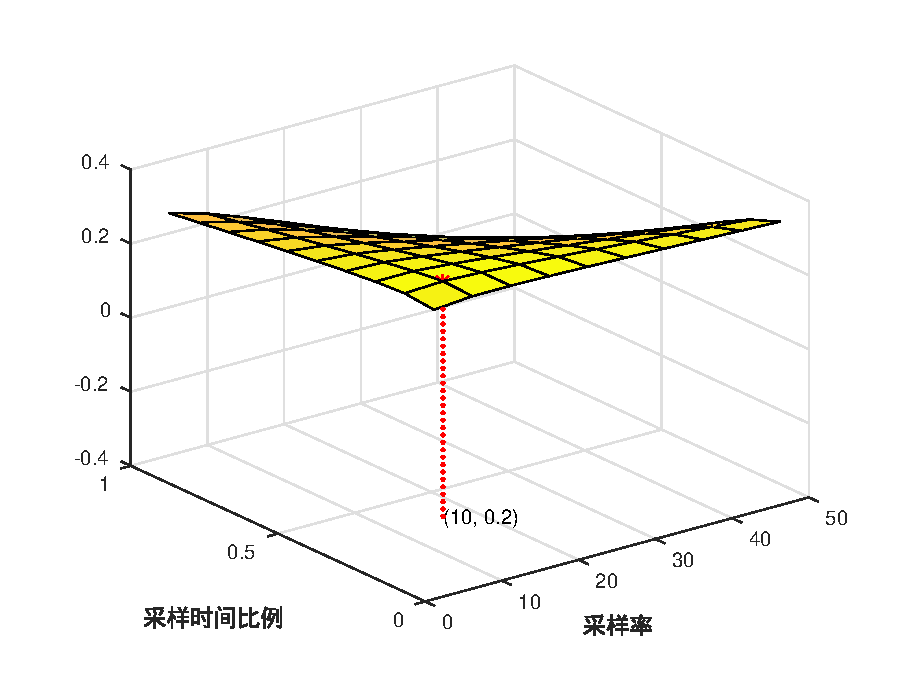
\includegraphics[width=0.3\textwidth]{object_run.eps}}
    \subfloat[上楼状态的目标函数]{
    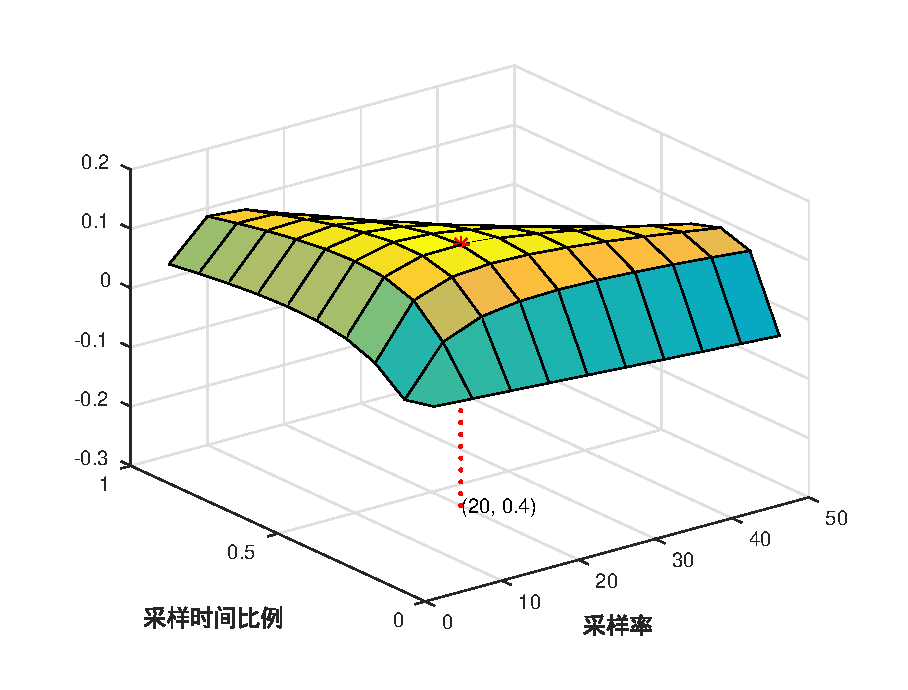
\includegraphics[width=0.3\textwidth]{object_ascend.eps}}
    \subfloat[下楼状态的目标函数]{
    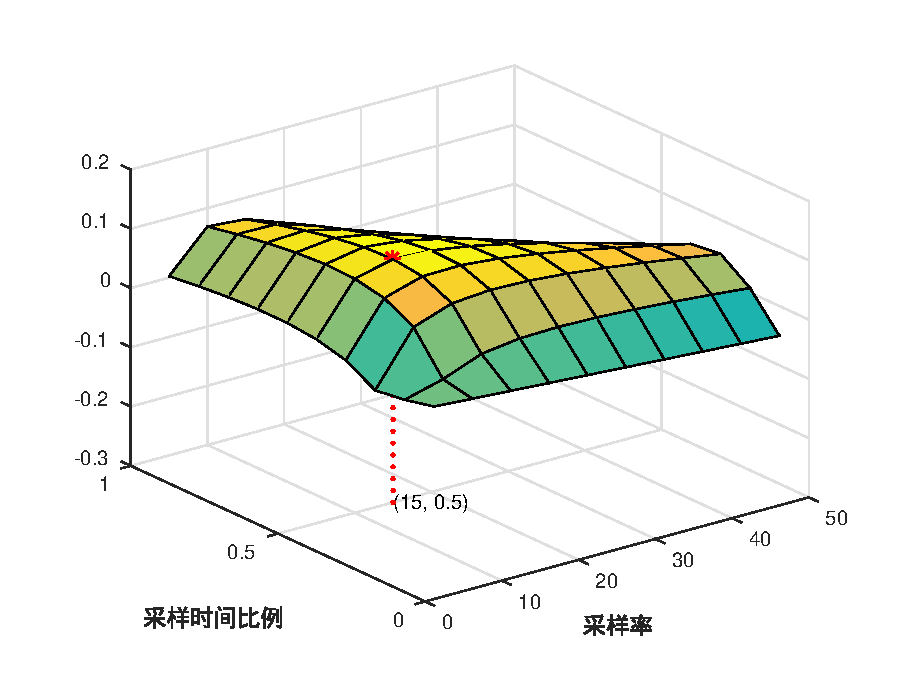
\includegraphics[width=0.3\textwidth]{object_descend.eps}}
    \caption{仅使用时域特征时各行为状态的目标函数}\label{object_function}
\end{figure}

\subsection{最优化问题求解}
\par 在通过实验测量求解获取能耗和准确率模型以后,就可以以当前电池电量等级为系数建立目标函数权衡二者关系,并通过求解关于目标函数的最优化问题就可以计算得到每类行为的最佳识别策略。本文中,目标函数的权衡系数是随着电量变化而动态调整的,通过当前电量的百分比,向上取10的整数倍计算权衡系数,取值为0.1到1.0十个动态选择的范围。对于目标函数中的两个离散变量,即是否使用频域和自相关函数特征,本文通过将目标函数分为四种情况分别计算其最优解,然后再对四个最优值比较选择最优解,同时也确定了最佳识别策略(\bm{$\widehat{f}$},\bm{$\widehat{\tau}$},\bm{$\widehat{\mu}$},\bm{$\widehat{\lambda}$}),其中采样率$\widehat{f_{ij}}$,采样时间比例$\widehat{\tau_{ij}}$,是否使用频域特征$\widehat{\mu_{ij}}$,是否使用自相关函数特征$\widehat{\lambda_{ij}}$,表示行为$i$在电量确定的权衡系数$\varphi (battery) = j/10$时的最佳识别策略。

\par 首先本文以仅使用时域特征时,并且考虑在设定电量权衡系数$\varphi (battery) = 0.5$的情况为例,计算目标函数。五类行为状态下,目标函数取反以后与采样率的和采样时间比例的函数关系如图\ref{object_function}(a)-(e)所示,其中在图中已经标出在仅使用时域特征时的各目标函数最优值以及其最佳采样率和采样时间比例。
%各行为状态下的目标函数图
\par 从图中可以看出,静止和跑步等区别较为明显的行为,对采样率和采样时间的依赖程度并不高,在较低的采样率和采样时间时具有较高的收益。而对于慢速动态行为,特别是上下楼时,当降低采样率和采样时间时到一定程度时,目标函数会急剧下降,说明此时的准确率降低的幅度较大,因此需要保证一定的采样率和采样时间。
\par 最后针对每一类行为求解目标函数的最优解,进而可以获得识别每一类行为的最佳策略,最佳策略如下表:
% 最佳策略表格
\begin{table}[htb]
    \centering
    \caption{各电量状态下各行为的最佳识别策略}
    \begin{tabular}{ccccccc}
    \toprule
    电量 & 静止 & 行走 & 跑步 & 上楼 & 下楼 \\
    \midrule
    10 & 10\%/5/T & 10\%/5/T & 10\%/5/T & 10\%/5/T & 10\%/5/T \\
    20 & 10\%/5/T & 10\%/10/TA & 10\%/5/T & 10\%/5/T & 10\%/5/T \\
    30 & 10\%/10/TA & 20\%/10/TA & 10\%/10/T & 30\%/10/TA & 30\%/5/TFA \\
    40 & 10\%/10/TA & 20\%/15/TA & 10\%/10/T & 30\%/10/TF & 40\%/5/TFA \\
    50 & 10\%/15/TA & 30\%/15/TA & 20\%/10/T & 40\%/10/TF & 50\%/5/TFA \\
    60 & 10\%/15/TA & 30\%/15/TA & 20\%/10/T & 50\%/10/TF & 60\%/5/TFA \\
    70 & 20\%/15/TA & 40\%/25/TA & 20\%/15/T & 60\%/10/TFA & 80\%/5/TFA \\
    80 & 20\%/15/TA & 50\%/25/TA & 30\%/15/T & 70\%/15/TF & 100\%/5/TFA \\
    90 & 20\%/25/TA & 60\%/25/TA & 30\%/15/TA & 100\%/15/TFA & 100\%/5/TFA \\
    100 & 30\%/25/TA & 70\%/50/TF & 40\%/15/TF & 1000\%/25/TFA & 100\%/5/TFA \\
    \bottomrule
    \end{tabular}
\end{table}

\par 其中每个策略的第一个变量是采样时间比例,第二个变量是采样率,单位是Hz,第三个是所使用的特征选择范围,T表示时域,F表示频域,A表示自相关函数有关的特征。从表格中可以看出,对于静止和跑步等区分较为明显的行为,采样时间不需要太长,所需要的特征也较为简单,而对于上楼和下楼区分不太明显的行为,则通常需要较长的采样时间,而且需要较多的特征,但是采样率要求不是太高。
\section{最佳策略动态调整方案}
\par 在计算获取到每种情况下的最佳策略以后,需要在人体行为识别过程中,根据上下文信息动态调整最佳策略,以实现降低识别过程中能耗的问题。首先,应用需要检测手机电量的变化,当电量变化会引起权衡系数变化时也就说明最佳策略也发生变化,此时需要作出线上实时调整。其次,应用需要根据当前的行为识别结果决定下一时刻的识别策略,其中最关键的问题在于判定行为的转变,即判定行为状态是否确定转变,需要对策略作出调整。为此,本文提出一种最佳策略的动态调整方案,其流程框图如图\ref{dapte_strategy}所示。
%最佳策略动态调整方法框图
\begin{figure}[ht]
\centering
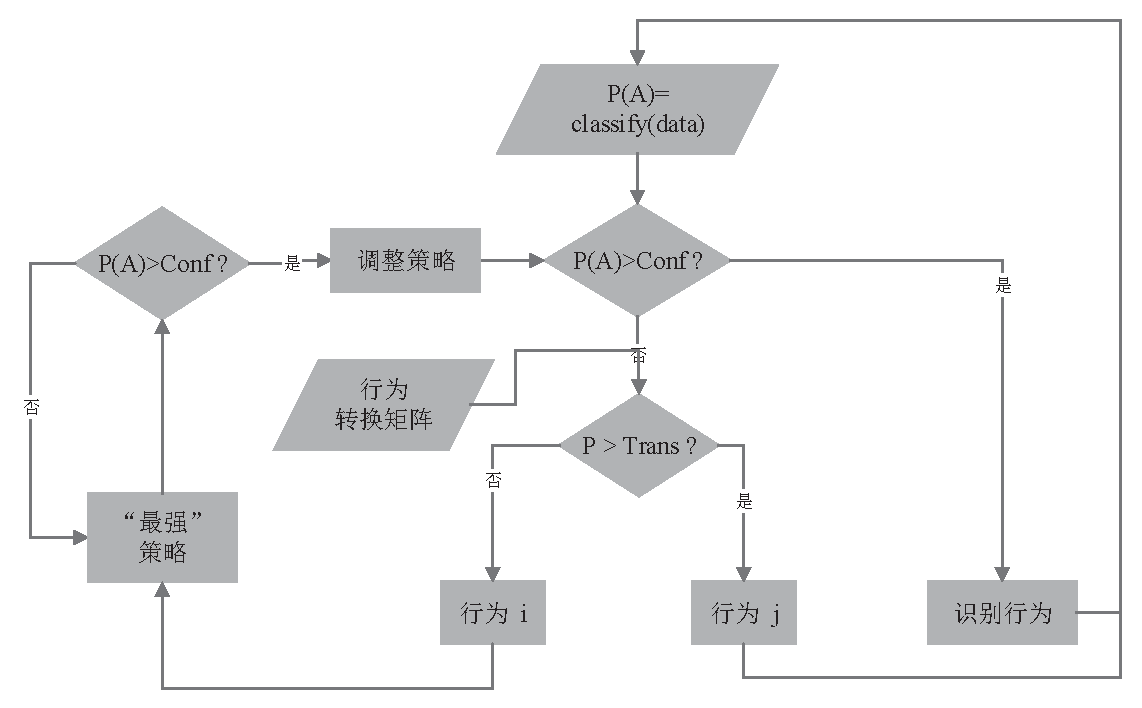
\includegraphics[width = 0.8\textwidth]{dapte_strategy.eps}
\caption{最佳策略的动态调整方案框图}\label{dapte_strategy}
\end{figure}

\par 在我们的识别框架中,分类方法继续使用前面介绍的随机森林的算法。随机森林分类方法通常会使用100棵决策树,每棵决策树从特征集中随机选择一定数量的特征组成特征向量进行决策分类,最后获得100个分类结果,随机森林算法将会选择其中比例最大的类别作为最终的分类结果。而在本文的方案框架将随机森林中所有决策树的识别结果中某类行为$j$所占的比例定义为$P(A_j)$, 表示分类器对该实例识别为行为$j$的概率, $Conf_{low}$为设定阈值,表示认为可以确定该行为的最低置信概率。若某一次识别过程中最终的识别行为的概率超过阈值$Conf_{low}$则确定为该识别结果,下一窗口时间使用该行为的最佳策略。若小于$Trans_{low}$,则计算实际行为转换概率$P_{ij}$当前行为$i$转换为行为$j$的概率,其计算公式可以表示为:
\begin{equation}
	max \{P_{ij} = P(A_j)a_{ij}\}, \quad j = 1 \cdots, i-1, i+1, \cdots, N
\end{equation}
其中, $i$表示前一次识别的行为,$a_{ij}$为行为转换矩阵中行为$i$转换为行为$j$的概率。若$P_{ij}$大于设定阈值$Trans_{low}$ ,则判定发生行为转变,下一窗口时间调整为行为$j$的最佳识别策略,否则,$P_{ij}$小于$Trans_{low}$则表示无法判定已经发生了明确的行为转换,此次判定为上一窗口的行为,即行为$i$,下一窗口时间使用“最强”识别方法,持续使用该策略识别,直到识别的概率超过阈值 ,则调整为对应行为的最佳策略,继续下一窗口的识别。

\section{对比实验结果}
\par 为了验证本文的最佳策略动态调整方案的有效性,我们通过实际生活中的监测实验,与没有使用最佳策略调整时的情况对比,分析最佳策略调整方案在能耗与准确率方面的性能。同时,本文也同之前的降低能耗的研究文献作出对比。在文献\cite{modelVarialb}中,作者研究了离散的识别策略调整方案,该文献中作者考虑了采样率和特征集的选择等变量,他们采用选择若干离散的采样率以及有限个数的特征集选择范围,然后将二者组成有限数量的二元组,最后通过权衡识别准确率和能耗,从中选择最佳的二元组最为最佳的识别策略。本小节剩余部分将通过对比实验作出本文方法与文献中方法的性能比较。

\subsection{实验设定}
\par 首先,该部分对比实验依然使用Google公司设计的Nexus5智能手机运行行为识别手机应用。实验对比对象为未实现策略动态调整的方案,离散的策略调整方案以及本文的动态调整方案,因此实验过程中有三部手机分别同时运行行为识别应用,其中第一部手机应用没有使用动态调整方案,后两部手机应用分别实现了文献\cite{}中和本文中的策略调整方案。实验的对比指标为应用的识别准确率和能耗两项。
\par 实验参与者同时佩戴三部手机分别运行上述三款应用,在没有干扰的情况下随机执行静止、行走、跑步、上楼和下楼五种类型的行为。为有效计算识别准确率,在实验过程中实时记录实验参与者的实际行为。实验的限定时间分别设置为10, 20, 30, 40, 50分钟,分别计算在限定时间内的准确率和能耗。本文实验共有6人参与,并计算准确率和能耗的平均值作为最终结果用于对比分析。
\subsection{实验结果与分析}
\par 行为识别手机应用在分别采用本文的最佳策略调整方案,离散的最佳策略调整方案\cite{modelVarialb}以及没有采用策略调整方案的情况下,同时对6人进行行为识别,相应的准确率和能耗的平均值分别表格\ref{final_precision}和\ref{final_energy},三类情况下的识别准确率和识别能耗如图\ref{com_result}所示。

\begin{table}[htb]
    \centering
    \caption{识别准确率}\label{final_precision}
    \begin{tabular}{ccccccc}
    \toprule
    时间 & 10 & 20 & 30 & 40 & 50 \\
    \midrule
    没有策略调整 & 0.9524 & 0.9637 & 0.9611 & 0.9680 & 0.9622 \\
    本文的策略调整 & 0.9294 & 0.9315 & 0.9394 & 0.9441 & 0.9440 \\
    离散的策略调整 & 0.9252 & 0.9288 & 0.9335 & 0.9306 & 0.9373 \\
    \bottomrule
    \end{tabular}
\end{table}

\begin{table}[htb]
    \centering
    \caption{识别能耗}\label{final_energy}
    \begin{tabular}{ccccccc}
    \toprule
    时间 & 10 & 20 & 30 & 40 & 50 \\
    \midrule
    没有策略调整 & 9.78 & 18.3 & 25.8 & 36.1 & 45.2 \\
    本文的策略调整 & 6.16 & 13.2 & 18.8 & 26.3 & 34.7 \\
    离散的策略调整 & 7.6567 & 15.6 & 19.9 & 27.9 & 38.6 \\
    \bottomrule
    \end{tabular}
\end{table}

\begin{figure}[!htb]
    \centering
    \subfloat[识别准确率]{
    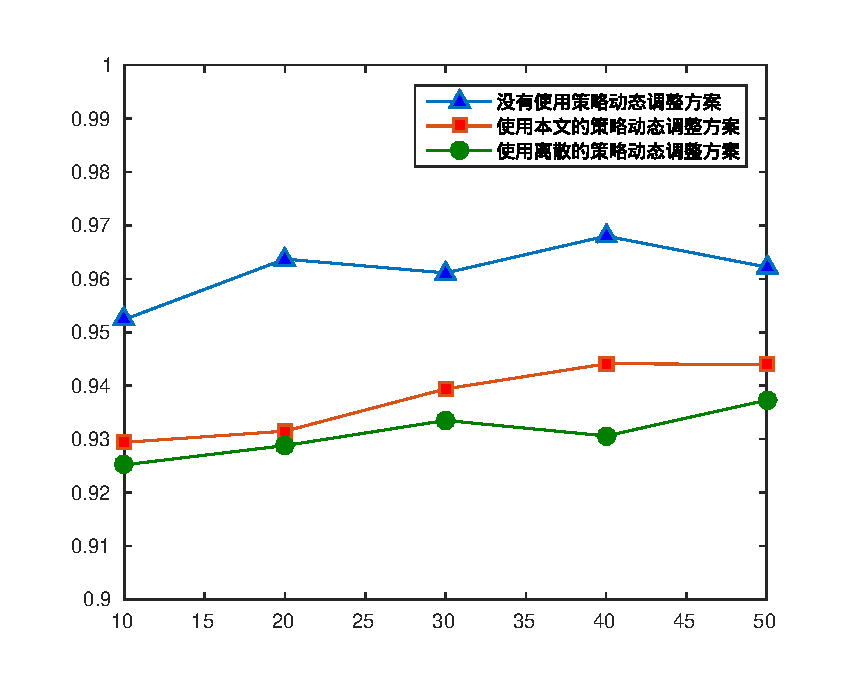
\includegraphics[width=0.45\textwidth]{precision.eps}}
    \subfloat[识别能耗]{
    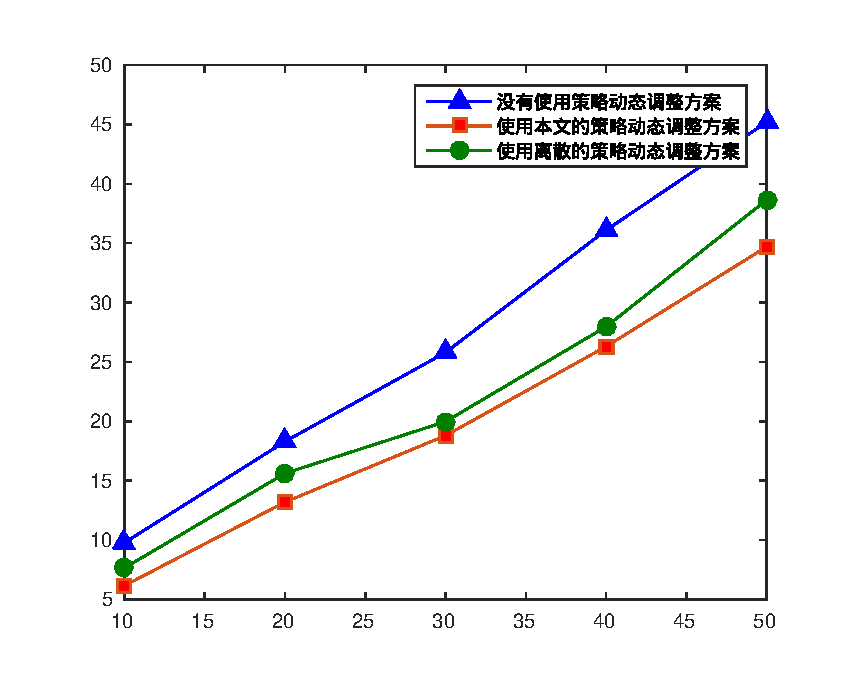
\includegraphics[width=0.45\textwidth]{energy.eps}}
    \caption{对比实验结果}\label{com_result}
\end{figure}

\par 如图\ref{com_result}所示,在使用策略动态调整的情况下,识别准确率有所下降,但是幅度不大,并且保持在90\%以上,而从图(b)可以看出在使用最佳策略调整的情况下,能耗有明显降低,相比与没有使用调整策略的情况,使用本文的策略调整方案能耗平均降低了28.48\%,而相比于之前的离散的策略调整方案,识别能耗也降低了11.43\%,从而说明了本文所提出最佳策略调整方案的有效性。

\section{本章小结}
\par 本章主要介绍了我们对降低行为识别过程中智能手机能耗的研究。降低能耗的基本思想是通过调节采样率等变量权衡行为识别过程中能耗与准确率之间的关系,进而选择一种最佳策略执行行为识别。本章首先对能耗和准确率建立了数学模型,研究二者与采样率、采样时间以及特征选择范围之间的函数关系,并以电量为权衡系数结合二者建立目标函数,从而将最佳策略选择转化为求解关于目标函数的最优化问题。然后通过实验测量的方法求解数学模型中的参数,为每一种行为求解出一种最佳的识别策略。同时,为了在识别过程中合理调整策略,本文介绍了一种结合行为转换和识别结果的转换判定方法,动态地调整最佳策略进行行为识别。最后,本章还通过设置对比实验分析了本文所提出的最佳策略动态调整方法的有效性。